\documentclass[12pt,a4paper]{report}
\usepackage[utf8]{inputenc}
\usepackage[spanish]{babel}
\usepackage{amsmath}
\usepackage{amsfonts}
\usepackage{amssymb}
\usepackage{makeidx}
\usepackage{graphicx}
\usepackage{lmodern}
\usepackage{kpfonts}
\usepackage[left=2cm,right=2cm,top=2cm,bottom=2cm]{geometry}
\author{Diego Armando Becerra Iñiguez}
\title{Angulos de Euler}
\begin{document}
\maketitle
El movimiento general de un sólido rígido posee 6 grados de libertad.

Por el teorema de Chasles, el movimiento general de un sólido puede descomponerse en una traslación de un punto seguida de una rotación del sólido alrededor de este punto (es decir,tomándolo como fijo en la rotación). Por ello, en la parametrización del movimiento de un sólido, estos 6 grados pueden descomponerse en 3 de traslación y tres de rotación.

Como grados de libertad de traslación basta dar el desplazamiento de un punto concreto del sólido (centro de reducción).

Para la rotación, en cambio, existen diferentes formas de parametrizarla, cada una con sus ventajas e inconvenientes. Así, tenemos:

-Dar directamente la matriz de rotación que pasa de un sistema de referencia ligado al sólido a uno exterior tomado como fijo. Esta matriz tiene 9 elementos sometidos a seis vínculos, lo cual multiplica el número de ecuaciones necesarias para la descripción del movimiento.

-Dar la orientación del eje de giro mediante dos ángulos (que pueden ser coordenadas esféricas, como la latitud y la longitud) y el ángulo de giro alrededor de este eje. Tiene el inconveniente, como los ángulos de Euler y otros, que requieren un abundante uso de funciones trigonométricas.

-Emplear los denominados parámetros de Euler que son un conjunto de cuatro variables, con un vínculo, que permiten representar toda matriz de rotación. Vienen a ser la generalización a 3 dimensiones de usar x e y para dar una rotación en el plano, sujetas a la condición $x^{2}+y^{2}=1$. Tienen el inconveniente de que no son fáciles de visualizar, aunque computacionalmente son muy eficientes.

-Emplear otros parámetros, como los de Cailey-Klein, que representan las rotaciones como operaciones sobre números complejos.

-Escribir la rotación general como una composición de tres rotaciones individuales sobre diferentes ejes. Esta es la técnica que se usa para definir los ángulos de Euler y los ángulos de navegación (o de Tait-Bryan). la diferencia entre los de Euler y los de Tait-Bryan es que en el primer caso se repite uno de los ejes, y en el segundo los tres ejes son diferentes. Los de Euler se emplean habitualmente al estudiar un movimiento planetario o el de un sólido con un punto fijo; los de navegación a la hora de indicar un posicionamiento de una aeronave o satélite.
\section{Ángulos de Euler}
Puede demostrarse que cualquier rotación de un sólido puede expresarse como la composición de tres rotaciones elementales alrededor de ejes diferentes (no necesariamente ortogonales). A su vez, estas rotaciones pueden considerarse en torno a unos ejes fijos o en torno a unos ejes intrínsecos.
\begin{figure}[hbtp]
\centering
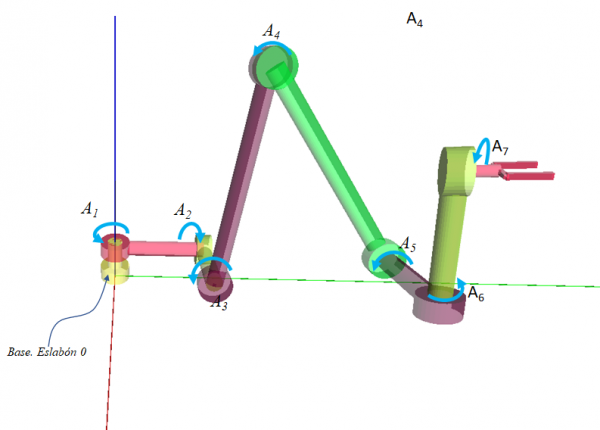
\includegraphics[width=4cm]{1.png}
\caption{Ejemplo de rotación}
\end{figure}

consideraremos la segunda opción, es decir, especificaremos una composición de rotaciones que nos llevarán desde un sistema exterior considerado fijo (“sólido 1”) hasta un sistema ligado al sólido (“sólido 4”) mediante sólidos intermedios. Para ello:

-Primero efectuamos una rotación de un ángulo $\varphi$ en torno a un eje del sólido 1 que nos lleva a un sólido intermedio “2”.

-A continuación rotamos un ángulo $\Theta$ en torno a un eje del sólido 2, que nos lleva a un sólido intermedio “3”.

-Por último, giramos un cierto ángulo $\psi$en torno a un eje del sólido 3, lo que nos lleva hasta el sólido móvil 4.

La elección de qué ejes son los de rotación puede hacerse de diferentes formas. La elección que haremos aquí, que es la más habitual en el uso de los ángulos de Euler consiste en la secuencia $z_{1}-x_{2}-z_{3}$ El que se repita uno de los ejes (aunque no sean coincidentes, por la rotación intermedia) es lo que define a esta descomposición como de ángulos de Euler. Si fueran todos diferentes ($z_{1}-y_{2}-x_{3}$,por ejemplo) serían de Tait-Bryan.

\section{Posición y matriz de rotación}
Para obtener el resultado de la rotación, debemos ver qué posición ocupa en el sistema de referencia fijo un punto perteneciente al sólido. El vector de posición se escribirá con componentes diferentes en la base fija y en la base móvil, aunque el vector sea el mismo.
\begin{center}
$\overrightarrow{OP}=\overrightarrow{r}=\overrightarrow{xi}+\overrightarrow{yi_{1}}+\overrightarrow{zk_{1}}=\overrightarrow{Xi_{4}}+\overrightarrow{yj_{4}}+\overrightarrow{Zk_{4}}$
\end{center}

donde, por ser un punto del sólido las componentes (X,Y,Z) son constantes. El problema se reduce entonces a relacionar los vectores de las bases. Para ello, componemos las tres rotaciones.

\section{Precisión}
La primera rotación es una de un ángulo $\phi$ entorno al eje $OZ_{1}=OZ_{2}$,que nos lleva al sólido 2. La relación entre la base fija 1 y la intermedia 2 es:
\begin{center}
 $\overrightarrow{i_{2}}=cos(\textrm \O)\overrightarrow{i_{1}}+sen(\textrm \O)\overrightarrow{j_{1}}$ 
 
 $\overrightarrow{j_{2}}=-sen(\textrm \O)\overrightarrow{i_{1}}+cos(\textrm \O)\overrightarrow{j_{2}}$
 
 $\overrightarrow{k_{2}}=\overrightarrow{k_{1}}$
 \end{center} 
Siendo su relacion inversa
\begin{center}
$\overrightarrow{i_{1}}=cos(\textrm \O)\overrightarrow{i_{2}}-sen(\textrm \O)\overrightarrow{j_{2}}$

$\overrightarrow{j_{1}}=sen(\textrm \O)\overrightarrow{i_{2}}+cos(\textrm \O)\overrightarrow{j_{2}}$

$\overrightarrow{k_{1}}=\overrightarrow{k_{2}}$
\end{center}
\begin{center}
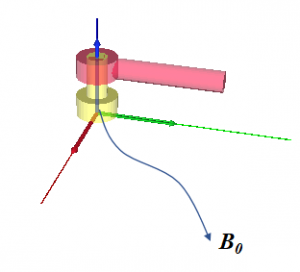
\includegraphics[width=4cm]{2.png}
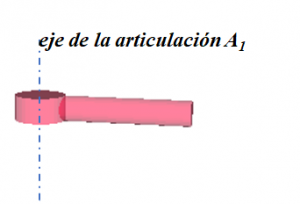
\includegraphics[width=4cm]{3.png} 
\end{center} 
A esta rotación, cuando se realiza sin modificar ninguno de los otros dos ángulos, se la denomina movimiento de precisión.
\section{Nutación}
La segunda rotación consiste en el giro de un ángulo $\theta$ alrededor del eje $OX_{2}=OX_{3}$ A este eje, que no se ve modificado por la rotación, se lo denomina línea de nodos. Esta rotación nos lleva al sólido intermedio 3, cuya base se relaciona con la 2 por:
\begin{center}
$\overrightarrow{i_{3}}=\overrightarrow{i_{2}}$

$\overrightarrow{j_{3}}=cos(\textrm \O)\overrightarrow{j_{2}}+sen(\textrm \O)\overrightarrow{k_{2}}$

$\overrightarrow{k_{3}}=-sen(\textrm \O)\overrightarrow{j_{2}}+cos(\textrm \O)\overrightarrow{k_{2}}$
\end{center}
Siendo su relación inversa:
\begin{center}
$\overrightarrow{i_{2}}=\overrightarrow{i_{3}}$

$\overrightarrow{j_{2}}=cos(\textrm \O)\overrightarrow{j_{3}}-sen(\textrm \O)\overrightarrow{k_{3}}$

$\overrightarrow{k_{3}}=sen(\textrm \O)\overrightarrow{j_{3}}+cos(\textrm \O)\overrightarrow{k_{3}}$
\end{center}
\begin{center}
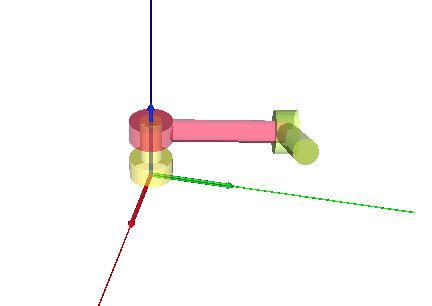
\includegraphics[width=4cm]{4.png}
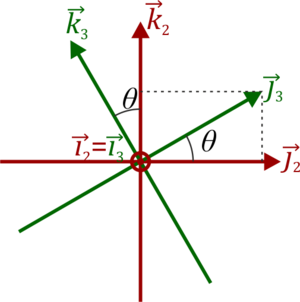
\includegraphics[width=4cm]{5.png} 

Cuando se produce esta rotación sin que se modifiquen las otras dos se dice que el sólido efectñua un movimiento de nutación.
\end{center} 
\section{Rotación propia}
El tercer giro (rotación propia, rotación intrínseca o simplemente rotación en el contexto del movimiento terrestre) corresponde a un nuevo giro de un ángulo $\Psi$ alrededor del ángulo $OX_{3}=OX_{4}$ (que no es el mismo, normalmente, que el $OX_{1}=OX_{2}$).La relación entre las bases 3 y 4 es análoga a la que hay entre la 1 y la 2.
\begin{center}
$\overrightarrow{i_{4}}=cos(\psi)\overrightarrow{i_{3}}+sen(\psi)\overrightarrow{j_{3}}$

$\overrightarrow{j_{4}}=-sen(\psi)\overrightarrow{i_{3}}+cos(\psi)\overrightarrow{j_{3}}$

$\overrightarrow{k_{4}}=\overrightarrow{k_{3}}$
\end{center}
Siendo su relación inversa:
\begin{center}
$\overrightarrow{i_{3}}=cos(\psi)\overrightarrow{i_{3}}-sen(\psi)\overrightarrow{j_{4}}$

$\overrightarrow{j_{3}}=sen(\psi)\overrightarrow{i_{4}}+cos(\psi)\overrightarrow{j_{4}}$

$\overrightarrow{k_{3}}=\overrightarrow{k_{4}}$
\end{center}
\begin{center}
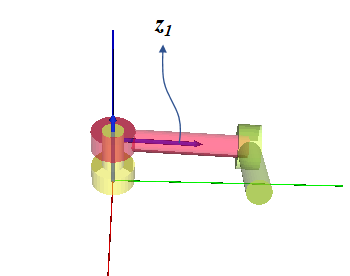
\includegraphics[width=4cm]{6.png}
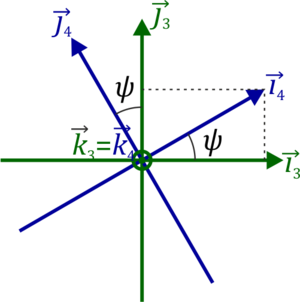
\includegraphics[width=4cm]{7.png} 
\end{center} 
El origen de los nombres precesión, nutación y rotación procede del análisis del movimiento terrestre. La rotación es el movimiento alrededor del eje terrestre. La precesión es el lento movimiento de dicho eje, que provoca que la estrella situada en el polo norte celeste vaya cambiando en el tiempo. La nutación es el cambio en la inclinación del eje terrestre, que no siempre ha estado a 23°27' como actualmente.
\begin{center}
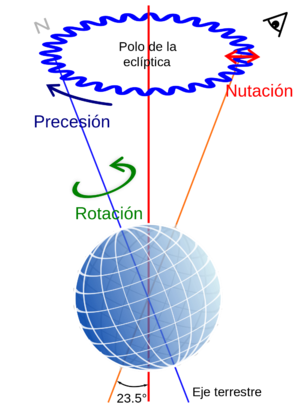
\includegraphics[width=4cm]{8.png} 
\end{center} 
\section{Matriz de rotación}
Para pasar directamente de la base 4, ligada al sólido, a la base 1, fija, podemos hacer sustituciones sucesivas, aunque los cálculos se vuelven rápidamente engorrosos. La matrix de rotación está formada por los productos escalares entre ambas bases.
\begin{center}
$\begin{pmatrix}
 a_{x} &\\ 
 a_{y} &\\
 a_{z} &
 \end{pmatrix}=\begin{pmatrix}
 {\overrightarrow{i_{1}}} & {\overrightarrow{i_{4}}} & {\overrightarrow{i_{1}}}& {\overrightarrow{j_{4}}}& {\overrightarrow{i_{1}}}& {\overrightarrow{k_{4}}}\\ 
 {\overrightarrow{j_{1}}} & {\overrightarrow{i_{4}}} & {\overrightarrow{j_{1}}}& {\overrightarrow{j_{4}}}& {\overrightarrow{j_{1}}}& {\overrightarrow{k_{4}}}\\ 
 {\overrightarrow{k_{1}}} & {\overrightarrow{i_{4}}} & {\overrightarrow{k_{1}}}& {\overrightarrow{j_{4}}}& {\overrightarrow{k_{1}}}& {\overrightarrow{k_{4}}}
 \end{pmatrix}*\begin{pmatrix}
 {x}&\\ 
 {y}&\\
 {z}&
 \end{pmatrix}$
\end{center}
siendo el camino más corto para hallar cada elemento no el pasar de la base 4 a la 1 directamente, sino ayudarnos de las bases intermedias. Así para el elemento R11 tenemos:

\begin{center}
$\overrightarrow{i_{1}}=cos(\phi)\overrightarrow{i_{2}}-sen(\phi)\overrightarrow{j_{2}}$

$\overrightarrow{i_{4}}=cos(\psi)\overrightarrow{i_{3}}+sen(\psi)\overrightarrow{j_{3}}$

$\overrightarrow{i_{1}}*\overrightarrow{i_{4}}=cos(\textrm \O)cos(\psi)\overrightarrow{i_{2}}*\overrightarrow{i_{3}}+cos(\textrm \O)sen(\psi)\overrightarrow{i_{2}}*\overrightarrow{j_{3}}-sen(\textrm\O)cos(\psi)\overrightarrow{j_{2}}*\overrightarrow{i_{3}}-sen(\textrm \O)sen(\psi)\overrightarrow{j_{2}}*\overrightarrow{j_{3}}$
\end{center}
y dado que,
\begin{center}
$\overrightarrow{i_{2}}*\overrightarrow{i_{3}}=1$

$\overrightarrow{i_{2}}*\overrightarrow{j_{3}}=\overrightarrow{j_{2}}*\overrightarrow{i_{3}}=0$

$\overrightarrow{j_{2}}*\overrightarrow{j_{3}}=cos(\theta)$

Queda finalmente:

$R_{11}=\overrightarrow{i_{1}}*\overrightarrow{i_{4}}=cos(\textrm \O)cos(\psi)-sen(\textrm\O)sen(\psi)cos(\theta)$
\end{center}

y análogamente para el resto de elementos. El más simple es.
\begin{center}
$R_{11}=\overrightarrow{k_{1}}*\overrightarrow{k_{4}}=\overrightarrow{k_{2}}*\overrightarrow{k_{3}}=cos(\theta)$
\end{center}
A estos resultados también se puede llegar multiplicando matrices, pero vamos a intentar aprovechar al máximo la cinemática del movimiento relativo.

\bibliographystyle{apalike}
\bibliography{biblio}
\end{document}